Cette section présente en \ref{par:contrib2_target} le problème cible, en \ref{par:contrib2_MoL} le schéma \texttt{I} méthode des lignes servant de référence et en \ref{par:paradigme_MRA} la façon dont la MRA est utilisée pour obtenir les schémas \texttt{II} et \texttt{III}.
\subsubsection{Problème cible}\label{par:contrib2_target}

    L'étude se fait en dimension un, l'équation d'évolution à résoudre est donc :
    \begin{align}
        \dt{u} = D \,\dxx{u} \quad D >0.
    \end{align}
    Les problématiques de bords ne sont pas prises en compte dans l'analyse.
        \subsubsection{Méthode des lignes utilisée}\label{par:contrib2_MoL}
            Pour résoudre cette équation aux dérivées partielles, une méthode des lignes est utilisée.\\
            \textbf{Discrétisation spatiale: }
            La discrétisation spatiale se fait à l'ordre deux selon le paradigme des volumes finis.
            L'équation est d'abord intégrée sur une cellule $C_k$ de taille $\Delta x$ centrée sur $x_k$ : 
            \begin{align}
                \int_{C_k} \dt{u}(x,t) \, dx = D \int_{C_k} \dxx{u}(x,t) \, dx 
            \end{align}
            Puis posant la valeur moyenne sur la cellule: $U_k(t) = \frac{1}{\Delta x} \int_{C_k} u(x,t) \, dx$ et en simplifiant l'intégrale de gauche:  
            \begin{align}
                \frac{d}{dt} U_k(t) = D \left[ \dx{u}(x_k + \frac{\Delta x}{2},t) - \dx{u}(x_k - \frac{\Delta x}{2},t)\right]
            \end{align}
            Puis en approximant les dérivées spatiales à l'ordre deux , cela donne l'équation semi-discrétisée en espace suivante.
            \begin{align}
                \dt{U}(t) = \frac{D}{\underbrace{\Delta x}_{\text{cellule}}} \Bigl(\frac{U_{k+1} - 2 U_{k} + U_{k-1}}{\underbrace{\Delta x}_{\text{approx. gradients}}}\Bigr)
            \end{align}
            On remarque que les $\Delta x$ qui apparaissent ont des origines distinctes, d'une part la taille de la cellule pour obtenir une valeur moyenne et 
            d'autre part la distance entre les deux points servant à approximer les gradients.\\
            \textbf{Intégration temporelle: } en notant $\mathbb{D}$ l'opérateur de diffusion spatial, l'intégration temporelle se fait grâce à la méthode Runge et Kutta explicite d'ordre deux suivant: 
            \begin{align}
                u^{n+1} = \left(Id+ \Delta t\, \mathbb{D} \ + \frac{1}{2} \, \Delta t^2 \, \mathbb{D}^2 \right) u^n.
            \end{align}
            C'est à dire:
            \begin{align}
                U_k^{n+1} &= U_k^n\\ \notag
                &+ D \frac{\Delta t}{\underbrace{\Delta x}_{\text{cellule}}} \Bigl(\frac{U_{k+1} - 2 U_{k} + U_{k-1}}{\underbrace{\Delta x}_{\text{approx. gradients}}}\Bigr)%\\ \notag
                +\frac{1}{2} \,D^2 \frac{\Delta t^2}{\underbrace{\Delta x^2}_{\text{cellule}}} \Bigl(\frac{U_{k+2} -4 U_{k+1}  +6 U_{k} -4 U_{k-1} + U_{k-2}}{\underbrace{\Delta x^2}_{\text{approx. gradients}}}\Bigr).
            \end{align}\\
            \textbf{Forme conservative: }
            Ce schéma peut s'écrire sous forme conservative en exhibant les flux numériques suivants :
            \begin{align}
                u^{n+1}_k = u^n_k +  D \frac{\Delta t}{\Delta x} \Bigl( \Phi^n_{k+1/2} - \Phi^n_{k-1/2} \Bigr)  + \left( D \frac{\Delta t}{\Delta x} \right)^2 \Bigl( \Psi^n_{k+1/2} - \Psi^n_{k-1/2} \Bigr) 
            \end{align}
            Avec:

            \begin{align}
                \Phi^n_{k+1/2} &= \frac{1}{\Delta x}(u^n_{k+1} - u^n_{k}),\\
                \Phi^n_{k-1/2} &= \frac{1}{\Delta x}(u^n_{k} - u^n_{k-1}),\\\notag
                \Psi^n_{k+1/2} &= \frac{1}{\Delta x^2} \left(\frac{1}{2} u^n_{k+2} -  \frac{3}{2}  u^n_{k+1} +  \frac{3}{2} u^n_{k} -  \frac{1}{2} u^n_{k-1}\right),\\\notag
                \Psi^n_{k-1/2} &= \frac{1}{\Delta x^2} \left(\frac{1}{2} u^n_{k+1} -  \frac{3}{2}  u^n_{k}   +  \frac{3}{2}u^n_{k-1} -  \frac{1}{2}u^n_{k-2}\right).\notag
            \end{align}
\newpage
        \subsubsection{La multirésolution adaptative, différents différents paradigmes ?}\label{par:paradigme_MRA}
            La multirésolution adaptative est présenté avec plus de détails en \ref{par:explication_MRA}.    
            Cette partie clarifie surtout la différence entre les deux schémas MRA étudiés (schémas \texttt{II} et \texttt{III}).
            Pour rappel, la multirésolution adaptative consiste à compresser la solution sur plusieurs niveau de profondeur,
            puis a effectuer les calculs sur la compressée.
            L'adaptation par MRA d'un schéma se fait de la manière suivante:
            \begin{enumerate}
                \item Partir d'un état compressé au pas de temps $n$.
                \item Calculer la solution au pas de temps $n+1$
                \item Compresser de nouveau selon un seuil de compression $\varepsilon$ grâce à une transformée multiéchelle et à l'heuristique d'Harten.
            \end{enumerate}
            La valeur d'une cellule à un niveau de détail donné est calculée au temps pas de temps suivant
            grâce à un flux numérique. 
            Cependant, la manière d'évaluer ce flux numérique n'est pas univoque et donc à plusieurs schémas numériques potentiels:
            \begin{itemize}
                \item[$\diamond$] Le schéma \texttt{II} calcule le flux numérique
                à partir des cellules voisines à l’interface évaluées au niveau de détail courant, c'est à dire au niveau de détail choisit par l'adaptation spatiale (voir \ref{fig:schema_algos}). 
                C'est la méthode dite \textit{sans reconstruction des flux}. C'est la paradigme classique en MRA.
                \item[$\diamond$] Le schéma \texttt{III} calcule le flux numérique 
                à partir des cellules voisines reconstruites au niveau de détail le plus fin (voir \ref{fig:schema_algos}). C'est la méthode dite \textit{avec reconstruction des flux au niveau le plus fin}.
                Cette approche n'est pas standard en MRA, elle est plus complexe à mettre en place et demande plus de calculs.
                Toutefois il est attendu que cela réduise l'erreur puisqu'elle permet d'évaluer le flux numérique à partir de valeurs plus précises.
                Pour des problèmes d'advection, ces gains ont été établis théoriquement et validé expérimentalement en \cite{belloti_et_al_2025}.
            \end{itemize}
        \begin{figure}[htpb]
\begin{center}
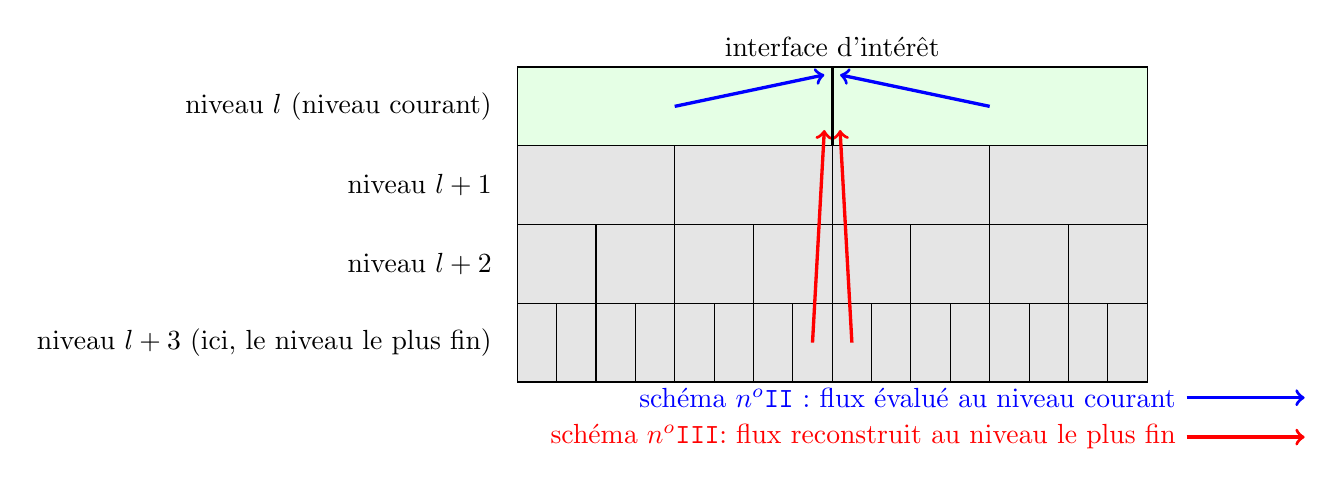
\begin{tikzpicture}
\foreach \i in {0,...,1}{
    \draw[fill=green!10] ({4*\i},0) rectangle ({4*(\i+1)},1);
}
\foreach \i in {0,...,3}{
    \draw[fill=black!10] ({2*\i},-1) rectangle ({2*(\i+1)},0);
}

\foreach \i in {0,...,7}{
    \draw[fill=black!10] ({\i},-2) rectangle ({(\i+1)},-1);
}

\foreach \i in {0,...,15}{
    \draw[fill=black!10] ({0.5*\i},-3) rectangle ({(.5*(\i+1))},-2);
}


\draw[blue, very thick, <-] (3.9,.9) -- (2,.5);
\draw[blue, very thick, <-] (4.1,.9) -- (6,.5);

% \draw[orange, very thick, <-] (3.9,.5) -- (3,-.5);
% \draw[orange, very thick, <-] (4.1,.5) -- (5,-.5);

\draw[red, very thick, <-] (3.9,.2) -- (3.75,-2.5);
\draw[red, very thick, <-] (4.1,.2) -- (4.25,-2.5);

\draw[black, very thick] (4,0) -- (4,1) node[pos=1, above] {interface d'intérêt};
\node[left] at (-.2,.5) {niveau $l$ (niveau courant)};
\node[left] at (-.2,-.5) {niveau $l+1$ };
\node[left] at (-.2,-1.5) {niveau $l+2$};
\node[left] at (-.2,-2.5) {niveau $l+3$ (ici, le niveau le plus fin)};

\draw[blue, very thick,->] (8.5,-3.2) -- (10,-3.2) node[pos=0,  left] {schéma $n^o$\texttt{II} : flux évalué au niveau courant};
\draw[red, very thick,->] (8.5,-3.7) -- (10,-3.7) node[pos=0,  left] {schéma $n^o$\texttt{III}: flux reconstruit au niveau le plus fin};
% \draw[orange, very thick,->] (8.5,-3.5) -- (10,-3.5) node[pos=0,  left] {algo 3. : flux reconstruit au niveau inférieur};


\end{tikzpicture}
\caption{Illustration de la différence entre les schémas adaptés spatialement \texttt{II} et \texttt{III}. Le schéma \texttt{II}
utilise l'information au niveau de détail $l$ pour calculer les flux numériques, c'est à dire l'information brute à l'issue de la compression.
En revanche, le schéma \texttt{III} reconstruit par interpolation polynomiale cette information au niveau de détail le plus fin, sur le schéma au niveau $l+3$.}
\label{fig:schema_algos}
\end{center}
\end{figure}
            Le travail suivant fournit donc les équations équivalentes du schéma \texttt{I} (non-adapté), 
            du schéma \texttt{II} (adapté, sans reconstruction des flux) et du schéma \texttt{III} (adapté, avec reconstruction des flux).
            Grâce à ces résultat, les erreurs théoriques portées par chacune de ces approches sont alors comparées et analysées.\par 

            \emph{Dans la suite seul le schéma \texttt{III} est détaillé par soucis de concision.}\\
            \textbf{L'opérateur de reconstruction}
            Étant donné une cellule à un niveau de détail donné $l$, on cherche à la faire évoluer du pas de temps $n$ vers le pas de temps $n+1$.
            A cette fin, évaluer les flux numérique doivent être évalués à partir les cellules voisines reconstruite par un 
            prédicteur à trois points (on dit qu'il à un \emph{stencil} de un, car il prend un compte une cellule de part et d'autre de la cellule centrale).\par
            L'opérateur de prédiction d'un niveau à l'autre s'écrit alors : 
            \begin{align}
                \hat u^{l+1}_{2k} &= +\frac{1}{8} u^l_{k-1} + u^l_k - \frac{1}{8} u^l_{k+1},\\
                \hat u^{l+1}_{2k+1} &= -\frac{1}{8} u^l_{k-1} + u^l_k + \frac{1}{8} u^l_{k+1}.
            \end{align}
            Puis en notant $\doublehat{u}^{l+\Delta l}_{(\cdot)}$ cet opérateur de prédiction itéré au travers de $\Delta l$ niveaux:
            \begin{align}
                \begin{bmatrix}
                    \doublehat{u}^{(l+\Delta l)}_{2^{\Delta l}k-2}\\
                    \doublehat{u}^{(l+\Delta l)}_{2^{\Delta l}k-1}\\
                    \doublehat{u}^{(l+\Delta l)}_{2^{\Delta l}k}\\
                    \doublehat{u}^{(l+\Delta l)}_{2^{\Delta l}k+1}\\
                \end{bmatrix}
                    =
                \underbrace{
                \begin{bmatrix}
                    +1/8 & 1 & -1/8 & 0 \\
                    -1/8 & 1 & +1/8 & 0 \\
                    0 & +1/8 & 1 & -1/8 \\
                    0 & -1/8 & 1 & +1/8 
                \end{bmatrix}^{\Delta l}}_{\text{Matrice de passage } P \text{ pour }s=1.}
                \cdot
                \begin{bmatrix}
                    u^l_{k-2}\\
                    u^l_{k-1}\\
                    u^l_{k}\\
                    u^l_{k+1}\\
                \end{bmatrix}
            \end{align}
\textbf{Flux reconstruits au niveau le plus fin: }
On travaille sur une cellule au niveau courant $l$ (de tailles $2^{\Delta l}\Delta x$) et l’on reconstruit les états au niveau $l+\Delta l$ grâce à des flux
flux au niveau fin, dont les gradients sont approximé par un pas $\Delta x$. La mise à jour conservative utilisée est donc
\begin{align}
u_k^{n+1}
= u_k^{n}
+ \frac{D\,\Delta t}{\underbrace{\Delta x\,2^{\Delta l}}_{\text{cellule}}}\Bigl(\doublehat{\Phi}_{k+\frac12}^n-\doublehat{\Phi}_{k-\frac12}^n\Bigr)
+ \left(\frac{D\,\Delta t}{\underbrace{\Delta x\,2^{\Delta l}}_{\text{cellule}}}\right)^2 \Bigl(\doublehat{\Psi}_{k+\frac12}^n-\doublehat{\Psi}_{k-\frac12}^n\Bigr).
\end{align}
Les flux sont évalués au \emph{niveau fin} (facteurs $1/\Delta x$ et $1/\Delta x^2$ portés par les flux) à partir d’états reconstruits $\doublehat{u}^{\,l+\Delta l}$ :
\begin{align}
\doublehat{\Phi}_{k-\frac12}^n
&= \frac{1}{\Delta x}\Bigl(
\doublehat{u}^{\,l+\Delta l}_{2^{\Delta l}k}
-\doublehat{u}^{\,l+\Delta l}_{2^{\Delta l}k-1}\Bigr),\\
\doublehat{\Phi}_{k+\frac12}^n
&= \frac{1}{\Delta x}\Bigl(
\doublehat{u}^{\,l+\Delta l}_{2^{\Delta l}(k+1)}
-\doublehat{u}^{\,l+\Delta l}_{2^{\Delta l}(k+1)-1}\Bigr),\\
\doublehat{\Psi}_{k-\frac12}^n
&= \frac{1}{\Delta x^2}\Bigl(
\tfrac12\,\doublehat{u}^{\,l+\Delta l}_{2^{\Delta l}k+1}
-\tfrac32\,\doublehat{u}^{\,l+\Delta l}_{2^{\Delta l}k}
+\tfrac32\,\doublehat{u}^{\,l+\Delta l}_{2^{\Delta l}k-1}
-\tfrac12\,\doublehat{u}^{\,l+\Delta l}_{2^{\Delta l}k-2}\Bigr),\\
\doublehat{\Psi}_{k+\frac12}^n
&= \frac{1}{\Delta x^2}\Bigl(
\tfrac12\,\doublehat{u}^{\,l+\Delta l}_{2^{\Delta l}(k+1)+1}
-\tfrac32\,\doublehat{u}^{\,l+\Delta l}_{2^{\Delta l}(k+1)}
+\tfrac32\,\doublehat{u}^{\,l+\Delta l}_{2^{\Delta l}(k+1)-1}
-\tfrac12\,\doublehat{u}^{\,l+\Delta l}_{2^{\Delta l}(k+1)-2}\Bigr).
\end{align}

\textbf{Forme matricielle du flux reconstruit: }
Pour simplifier l'usage les outils de calculs formels, il est pertinent d'écrire se qui précède sous forme matricielle.\\
Pour les flux gauches:
\begin{align}
\doublehat{\Phi}_{k-\frac12}^n
&= \frac{1}{\Delta x}\,
\begin{bmatrix}0 \\ -1 \\ +1 \\ 0\end{bmatrix}^\top \cdot
\begin{bmatrix}
\frac{1}{8} & 1 & -\frac{1}{8} & 0\\
-\frac{1}{8} & 1 & +\frac{1}{8} & 0\\
0 & +\frac{1}{8} & 1 & -\frac{1}{8}\\
0 & -\frac{1}{8} & 1 & +\frac{1}{8}
\end{bmatrix}^{\!\Delta l} \cdot
\begin{bmatrix}
u^l_{k-2}\\ u^l_{k-1}\\ u^l_{k}\\ u^l_{k+1}
\end{bmatrix},\\
\doublehat{\Psi}_{k-\frac12}^n
&= \frac{1}{\Delta x^2}\,
\begin{bmatrix}-\tfrac12 \\ +\tfrac32 \\ -\tfrac32 \\ +\tfrac12\end{bmatrix}^\top \cdot
\begin{bmatrix}
\frac{1}{8} & 1 & -\frac{1}{8} & 0\\
-\frac{1}{8} & 1 & +\frac{1}{8} & 0\\
0 & +\frac{1}{8} & 1 & -\frac{1}{8}\\
0 & -\frac{1}{8} & 1 & +\frac{1}{8}
\end{bmatrix}^{\!\Delta l} \cdot
\begin{bmatrix}
u^l_{k-2}\\ u^l_{k-1}\\ u^l_{k}\\ u^l_{k+1}
\end{bmatrix}.
\end{align}
Pour les flux droits:
\begin{align}
\doublehat{\Phi}_{k+\frac12}^n
&= \frac{1}{\Delta x}
\begin{bmatrix}0 \\ -1 \\ +1 \\ 0\end{bmatrix}^\top \cdot
\begin{bmatrix}
\frac{1}{8} & 1 & -\frac{1}{8} & 0\\
-\frac{1}{8} & 1 & +\frac{1}{8} & 0\\
0 & +\frac{1}{8} & 1 & -\frac{1}{8}\\
0 & -\frac{1}{8} & 1 & +\frac{1}{8}
\end{bmatrix}^{\!\Delta l} \cdot
\begin{bmatrix}
u^l_{k-1}\\ u^l_{k}\\ u^l_{k+1}\\ u^l_{k+2}
\end{bmatrix},\\
\doublehat{\Psi}_{k+\frac12}^n
&= \frac{1}{\Delta x^2}
\begin{bmatrix}-\tfrac12 \\ +\tfrac32 \\ -\tfrac32 \\ +\tfrac12\end{bmatrix}^\top \cdot
\begin{bmatrix}
\frac{1}{8} & 1 & -\frac{1}{8} & 0\\
-\frac{1}{8} & 1 & +\frac{1}{8} & 0\\
0 & +\frac{1}{8} & 1 & -\frac{1}{8}\\
0 & -\frac{1}{8} & 1 & +\frac{1}{8}
\end{bmatrix}^{\!\Delta l} \cdot
\begin{bmatrix}
u^l_{k-1}\\ u^l_{k}\\ u^l_{k+1}\\ u^l_{k+2}
\end{bmatrix}.
\end{align}


            % En particulier, si la cellule étudiée est au niveau courant $l$ alors on choisira d'aller approximer le flux au niveau le plus fin, c'est à dire avec $\dlbar = \bar l - l$.
            % Dès lors les flux approximés au niveau fins sont : 
            % \begin{align}
            %     \doublehat{\Phi}_{k-1/2} &= \doublehat{u}^{l+\dlbar}_{2^{\dlbar} k} -  \doublehat{u}^{l+\dlbar}_{2^{\dlbar} k-1} + \frac{1}{2} \lambda 
            %     \Bigl(
            %         \doublehat{u}^{l+\dlbar}_{2^{\dlbar} k+1}
            %         - 3 \doublehat{u}^{l+\dlbar}_{2^{\dlbar} k}
            %         + 3 \doublehat{u}^{l+\dlbar}_{2^{\dlbar} k-1}
            %         - \doublehat{u}^{l+\dlbar}_{2^{\dlbar} k-2}
            %     \Bigr),\\
            %     \doublehat{\Phi}_{k+1/2} &=  \doublehat{u}^{l+\dlbar}_{2^{\dlbar} (k+1)} -  \doublehat{u}^{l+\dlbar}_{2^{\dlbar} (k+1)-1} + \frac{1}{2} \lambda \Bigl(
            %         \doublehat{u}^{l+\dlbar}_{2^{\dlbar} (k+1)+1}
            %         - 3 \doublehat{u}^{l+\dlbar}_{2^{\dlbar} (k+1)}
            %         + 3 \doublehat{u}^{l+\dlbar}_{2^{\dlbar} (k+1)-1}
            %         - \doublehat{u}^{l+\dlbar}_{2^{\dlbar} (k+1)-2}
            %     \Bigr)
            % \end{align}
            
            % Cela s'écrit sous la forme matricielle suivante (utile pour utiliser les outils de calcul formel).
            % \begin{align}
            %     \doublehat{\Phi}_{k-1/2}
            %         &=
            %     \begin{bmatrix}
            %         -\frac{\lambda}{2}&
            %         (\frac{3}{2} \lambda - 1)&
            %         (1 - \frac{3}{2} \lambda)&
            %         \frac{\lambda}{2}&
            %     \end{bmatrix}
            %     \begin{bmatrix}
            %         +1/8 & 1 & -1/8 & 0\\
            %         -1/8 & 1 & +1/8 & 0\\
            %         0 & +1/8 & 1 & -1/8\\
            %         0 & -1/8 & 1 & +1/8\\
            %     \end{bmatrix}^{\dlbar}
            %     \begin{bmatrix}
            %         u^l_{k-2}\\
            %         u^l_{k-1}\\
            %         u^l_{k}\\
            %         u^l_{k+1}\\
            %     \end{bmatrix}
            % \end{align}
            % \begin{align}
            %     \doublehat{\Phi}_{k+1/2}
            %         &=
            %     \begin{bmatrix}
            %         -\frac{\lambda}{2}&
            %         (\frac{3}{2} \lambda - 1)&
            %         (1 - \frac{3}{2} \lambda)&
            %         \frac{\lambda}{2}&
            %     \end{bmatrix}
            %     \begin{bmatrix}
            %         +1/8 & 1 & -1/8 & 0\\
            %         -1/8 & 1 & +1/8 & 0\\
            %         0 & +1/8 & 1 & -1/8\\
            %         0 & -1/8 & 1 & +1/8\\
            %     \end{bmatrix}^{\dlbar}
            %     \begin{bmatrix}
            %         u^l_{k-1}\\
            %         u^l_{k}\\
            %         u^l_{k+1}\\
            %         u^l_{k+2}\\
            %     \end{bmatrix}.
            % \end{align}

            % Attention le schéma final est légèrement différent car il fait ici intervenir deux pas d'espace: $\Delta x$ le pas au niveau le plus fin
            % et $\Tilde {\Delta x} = 2^{\Delta l} \Delta x$ le pas du niveau courrant. Ainsi le schéma final est :
            % \begin{align}
            %     {u}^{n+1}_k = {u}^n_k + \frac{\lambda}{2^{\Delta l}} \Bigl( \doublehat{\Phi}^n_{k+1/2} - \doublehat{\Phi}^n_{k-1/2} \Bigr)
            % \end{align}